\section{Durchführung}
\label{sec:Durchführung}
In Abbildung \ref{fig:acrylblock} ist der Acrylglasblock, im Folgenden als Acrylblock bezeichnet,
der genauer untersucht wird, zu sehen. Inbesondere sind dort die Fehlstellen nummeriert, sodass
sie nach diesem Verfahren im weiteren Verlauf referenziert werden.

\begin{figure}
  \centering
  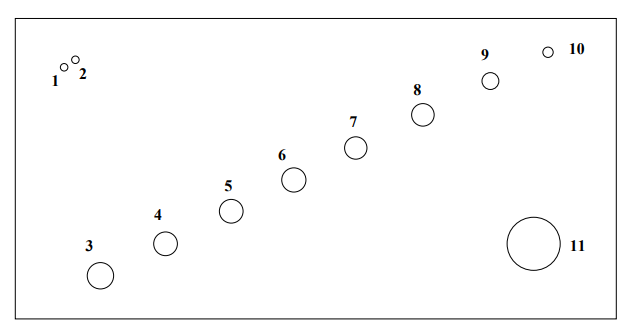
\includegraphics[width=\textwidth]{data/acrylblock.png}
  \caption{Bezeichnungen der Fehlstellen im Acrylblock\,\cite{Versuchsanleitung}}
  \label{fig:acrylblock}
\end{figure}

Zunächst werden die Abmessungen des Acrylblocks mit einer Schieblehre bestimmt.
Dazu werden die Durchmesser und Lagen der Fehlstellen in beiden
möglichen Orientierungen des Acrylblocks gemessen. Die Messung der Lage bedeutet, dass
die Entfernung des oberen Endes der Fehlstelle zum oberen Ende des Blocks sowie die
Entfernung des unteren Endes der Fehlstelle zum Boden des Blocks gemessen wird.

Danach wird der Acrylblock auf ein Papiertaschentuch gestellt und als Kontaktmittel
bidestilliertes Wasser auf seine Oberseite gegeben. Seine Orientierung ist genauso wie in
der obigen Abbildung. Eine blaue Sonde mit einer Frequenz von 1\,MHz wird an das
Ultraschallechoskop angeschlossen. Dieses ist mit einem Computer verbunden, sodass
die Daten graphisch dargestellt werden können. Durch Eingabe der Schallgeschwindigkeit
in Acryl von $c_\text{A} = \SI{2730}{\meter\per\second}$(QUELLENANGABE!) in das Programm ist auf der Abszisse die
Entfernung von der Sonde bereits angegeben. Auf der Ordinate ist die Amplitude des Echos
aufgetragen. Durch Bewegung der Sonde über die einzelnen Fehlstellen kann dann eine
Entfernung abgelesen werden. Für die Fehlstellen der Nummern 1 und 2 werden Bilder mithilfe
des Computers angefertigt, um später das Auflösungsvermögen Ultraschallsonden verschiedener
Frequenzen zu diskutieren. Der A-Scan wird wiederholt, nachdem der Block umgedreht wurde.\\
Zudem wird mit einer 4\,MHz-Sonde ein A-Scan von den Störstellen 1 und 2 von beiden Seiten
gemacht und jeweils ein Bild gespeichert.
%Vielleicht noch welche Sonde für was genau genommen wurde... gucke ich morgen im Heft nach...
Daraufhin wird mit einer 2\,MHz-Sonde ein B-Scan des Acrylblocks durchgeführt. Die Sonde wird dafür mit einer
möglichst konstanten Geschwindigkeit über den Block geführt. Aus den Bildern, die
der Computer generiert, können Werte für die Lagen der Störstellen abgelesen werden.

Zuletzt wird ein Herzmodell, welches aus zwei durch eine Membran getrennten Zylindern
besteht, mit einer 2\,MHz-Sonde untersucht. Durch einen Gummiball kann dem unteren Zylinder Luft zugeführt werden, sodass die Membran
sich erhebt. In den oberen Zylinder wird Wasser eingefüllt und die Ultraschallsonde
wird so fixiert, dass sie gerade so in das Wasser eintaucht. Mit einem A-Scan wird die
Entfernung bis zur Membran bestimmt, dies wird auch für eine gewölbte Membran gemacht.
Dafür wird im Programm die Schallgeschwindigkeit von destilliertem Wasser
$c_\text{W}=\SI{1485}{\meter\per\second}$(QUELLENANGABE!) eingetragen.
Nun wird ein TM-Scan durchgeführt. Dazu wird möglichst regelmäßig Luft in das Modell
gepumpt und abgelassen, sodass das Schlagen eines Herzens simuliert wird. Aus dem
sich ergebenden Bild werden später Informationen ermittelt, weswegen das Bild gespeichert wird.
